\subsection{Hjørner}\label{subsec:corner}
At detektere hjørner er en udbredt teknik indenfor feature detektion, da hjørner ofte forekommer i forskellige menneskeskabte scener og fordelagtigt kan bruges i disse sammenhæng.
Et hjørne kan defineres som et område i og omkring et punkt, der har to dominerede kantretninger (beskrevet i sektion ref). Der opstår derved store intensitetsvariationer i områder, hvor der forekommer hjørner.
Den store intensitetsvariation medføre at hjørner er distinktive og derved kan bruges som interessepunkter. En intuitiv måde at bestemme om et område er distinktivt er ved at sammenligne området, med naboliggende områder. Er området ens med de omkringliggende områder, er området ikke distinkt. Er området forskelligt, kan dette område unikt udvælges og er derved distinktivt.
\begin{figure}[H]
    \centering
    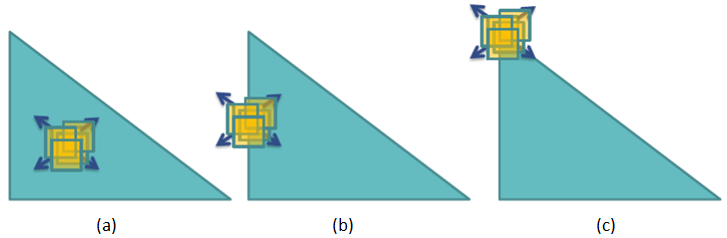
\includegraphics[width=0.75\textwidth]{fig/6.png}
    \vspace{-1em}   
    \begin{center}    
    \caption{\textcolor{gray}{\footnotesize \textit{
     Tre udvalgte vinduer, med interessepunkter i centrum af samme motiv. \textbf{(a)} Punktet er lokaliseret i en teksturløs region, d.v.s. ingen teksturskift. \textbf{(b)} Punktet er lokaliseret på en kant. \textbf{(c)} Punktet er lokaliseret på et hjørne }}}
    \label{fig:2}
     \end{center}
    \vspace{-2.7em}  
  \end{figure}  
\noindent
Et eksempel på ovenstående definition er illustreret i figur \ref{fig:2}, hvor tre punkter er udvalgt med et dataindsamlingsvindue placeret henover. For at bestemme om punkternes områder er distinktive, forskydes dataindsamlingsvindue med en enkelt pixel i de otte principielle retninger. Vil et af de otte forskudte vinduer portrættere den samme scene som det originale vindue omkring punktet, er punktet ikke distinkt. Forskydes  \textbf{(a)} vil alle de forskudte vinduer være ens med det originale, da området omkring er fladt. Det vil ikke være muligt at udvælge to korresponderende punkter på flade regioner.
Forskydes \textbf{(b)} i x-aksen vil der opstå et vindue der er forskelligt fra det originale, men en forskydning i y-aksen vil resultere i et vindue, ens med det originale. Et interessepunkt placeret her vil ikke kunne differentieres fra punkter lokaliseret langs y-aksen og er derved ikke distinkt. Punktet placeret på et hjørne \textbf{(c)} er interessant da forskydninger uanset retning, vil resultere i en region, der ikke er identisk med den originale. Et punkt placeret her vil derved kunne differentieres fra eventuelt omkringliggende punkter, og kan derved bruges som et interessepunkt. Figur \ref{app} illustrere ovenstående nævnte problemstillinger ved udvælgelsen af korrespondancer i ikke distinktive regioner.
\begin{figure}[H]
    \centering
    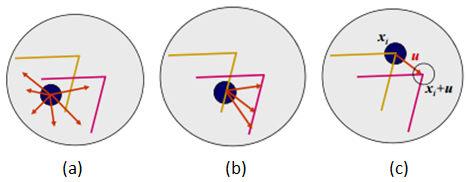
\includegraphics[width=0.55\textwidth]{fig/37.png}
    \vspace{-1em}   
    \begin{center}    
    \caption{\textcolor{gray}{\footnotesize \textit{
 }}}
    \label{app}
     \end{center}
    \vspace{-2.7em}  
  \end{figure}  
\noindent
Denne intuitive definition af et hjørne kan kvantificeres til en matematisk definition, der estimere auto-korrelationen imellem de forskudte billeder, hvilket angiver intensitetsvariationen imellem billederne og derved angiver hvor der opstår et hjørne.
\\ \\
Ovenstående udleder at områderne omkring hjørner er distinktive, og udvælges en begrænset mængde hjørner i billedet, vil det leve op til en repeterbar detektion.

Hvis det antages, at der forekommer en begrænset mængde hjørner i et billede, kan et hjørne bruges som interessepunkt, da lever op til kravet om repeterbarhed. <Om det er distinktivt, kan diskuteres>.